\documentclass{sigchi}

% Use this command to override the default ACM copyright statement (e.g. for preprints). 
% Consult the conference website for the camera-ready copyright statement.


%% EXAMPLE BEGIN -- HOW TO OVERRIDE THE DEFAULT COPYRIGHT STRIP -- (July 22, 2013 - Paul Baumann)
% \toappear{Permission to make digital or hard copies of all or part of this work for personal or classroom use is 	granted without fee provided that copies are not made or distributed for profit or commercial advantage and that copies bear this notice and the full citation on the first page. Copyrights for components of this work owned by others than ACM must be honored. Abstracting with credit is permitted. To copy otherwise, or republish, to post on servers or to redistribute to lists, requires prior specific permission and/or a fee. Request permissions from permissions@acm.org. \\
% {\emph{CHI'14}}, April 26--May 1, 2014, Toronto, Canada. \\
% Copyright \copyright~2014 ACM ISBN/14/04...\$15.00. \\
% DOI string from ACM form confirmation}
%% EXAMPLE END -- HOW TO OVERRIDE THE DEFAULT COPYRIGHT STRIP -- (July 22, 2013 - Paul Baumann)


% Arabic page numbers for submission. 
% Remove this line to eliminate page numbers for the camera ready copy
\pagenumbering{arabic}


% Load basic packages
\usepackage{balance}  % to better equalize the last page
\usepackage{graphics} % for EPS, load graphicx instead
\usepackage{times}    % comment if you want LaTeX's default font
\usepackage{url}      % llt: nicely formatted URLs


% llt: Define a global style for URLs, rather that the default one
\makeatletter
\def\url@leostyle{%
  \@ifundefined{selectfont}{\def\UrlFont{\sf}}{\def\UrlFont{\small\bf\ttfamily}}}
\makeatother
\urlstyle{leo}


% To make various LaTeX processors do the right thing with page size.
\def\pprw{8.5in}
\def\pprh{11in}
\special{papersize=\pprw,\pprh}
\setlength{\paperwidth}{\pprw}
\setlength{\paperheight}{\pprh}
\setlength{\pdfpagewidth}{\pprw}
\setlength{\pdfpageheight}{\pprh}


% Make sure hyperref comes last of your loaded packages, 
% to give it a fighting chance of not being over-written, 
% since its job is to redefine many LaTeX commands.
\usepackage[pdftex]{hyperref}
\hypersetup{
pdftitle={SIGCHI Conference Proceedings Format},
pdfauthor={LaTeX},
pdfkeywords={SIGCHI, proceedings, archival format},
bookmarksnumbered,
pdfstartview={FitH},
colorlinks,
citecolor=black,
filecolor=black,
linkcolor=black,
urlcolor=black,
breaklinks=true,
}

% create a shortcut to typeset table headings
\newcommand\tabhead[1]{\small\textbf{#1}}


% End of preamble. Here it comes the document.
\begin{document}

\title{Brainstorming In the Crowd:\\*Ask for More Than 20 Ideas}

\numberofauthors{1}
\author{
  \alignauthor Anonymous for Review\\
  \affaddr{~}\\
    \affaddr{~}\\
    \email{~}\\
    \affaddr{~}    
}

\maketitle

\begin{abstract}
Microtask marketplaces enable hybrid computational systems that use crowds to solve problems of creativity, such as brainstorming. We present a first characterization of brainstorming in this context, providing models for the rate of idea generation, the rate of category generation and the originality of generated ideas. We demonstrate that the rates of idea and category generation can be closely fit by a logarithmic model, and show that the first few responses of a brainstorming run are drawn from a pool of very common, obvious ideas. Our results suggest that ideas become more original after 20 ideas have been collected. Furthermore, we explore the phenomenon of \emph{riffing} in brainstorming tasks, and replicate two related findings from prior work. Our results provide recommendations for those leveraging the crowd for brainstorming, and comparable models of creative idea generation research community.


%Microtask marketplaces enable hybrid computational systems that use crowds to solve problems of creativity, such as brainstorming. We present a first characterization of brainstorming in this context, providing models for the rate of idea generation, the rate of category generation, the originality of ideas and the novelty of ideas. We demonstrate that the rates of idea and category generation can be closely fit by a logarithmic model, that these rates roughly increase if fewer participants are asked for more responses, and that this distinction is the result of a \emph{burn in period}  of common ideas at the beginning of a brainstorming task. Furthermore, we explore the phenomenon of \emph{riffing} in brainstorming tasks, and replicate two related findings from prior work. Our results provide recommendations for those leveraging the crowd for brainstorming, and comparable models of creative idea generation research community.

\end{abstract}

\keywords{
  Brainstorming, crowdsourcing, Mechanical Turk
}

\category{H.5.m.}{Information Interfaces and Presentation (e.g. HCI)}{Miscellaneous}

\section{Introduction}
This format is to be used for submissions that are
published in the conference proceedings.  We wish to give
this volume a consistent, high-quality appearance. We
therefore ask that authors follow some simple
guidelines. In essence, you should format your paper
exactly like this document. The easiest way to do this is
simply to download a template from the conference web
site, and replace the content with your own material.




\section{Related Work}
In this section, we review related work in the areas of brainstorming and crowdsourcing.

\subsection{Traditional Brainstorming}
In the 1950s, Osborne formalized the brainstorming process, providing a set of recommendations for idea generation by groups \cite{osborn_applied_1957}: \emph{focus on quantity}, \emph{withhold criticism}, \emph{welcome unusual ideas}, and \emph{combine and improve ideas}. These recommendations form the basis for the instructions we provide to workers in our experiments.

Following Osborne's work, Taylor et al.\ established that brainstorming by \emph{nominal groups}, or individuals working in isolation from one another, yields better results than collocated groups in terms of number of ideas generated \cite{taylor_does_1958}. These effects can be partially explained by the absence of counterproductive social forces, such as fear of judgment. Bouchard and Hare \cite{bouchard_jr_size_1970} later found that nominal brainstorming groups are able to generate quantities of ideas linear in the number of members in the group.

Electronic brainstorming is a variant in which individuals brainstorm at separate computer terminals, with the exchange of ideas performed over the network \cite{gallupe_electronic_1992}. Participants enter ideas while others' ideas are anonymously presented on-screen. As with nominal brainstorming, Gallupe \cite{gallupe_electronic_1992} observed that electronic brainstorming can reduce counterproductive social effects. However, Pinsonneault et al.\ \cite{pinsonneault_electronic_1999} identify productivity impediments introduced by group electronic brainstorming, such as being distracted by other ideas appearing, and individuals witholding ideas they feel are derivative of others. They find little evidence to support the proposition that electronic brainstorming outperforms nominal brainstorming.

Finally, Diehl and Stroebe found that groups that generate many ideas also generate \emph{good} ideas \cite{diehl_productivity_1987}, a finding that has been verified many times \cite{briggs1997quality, parnes1959effects, parnes_effects_1961, shah2003metrics, cross1996creativity}.

Shifting our focus to an \emph{individual's} brainstorming processes, Nijstad and Stroebe provide a model for individual idea generation dubbed SIAM, or the ``search for ideas in associative memory'' \cite{nijstad_how_2006}. SIAM defines two stages of idea generation: the generation of ideas based on working memory, and idea production within a single activated ``image'' (where an image can be thought of as a category of ideas). This model makes predictions, one of the most important being that an idea is more likely to be followed by an idea in the same category than would be expected by chance. Their model also predicts that new ideas in the same category as the previous idea are generated faster than ideas between categories. Nijstad and Stroebe verified these predictions in the context of nominal brainstorming.

To assess the brainstorming process and its outputs, a number of measures have been proposed. Typically, the measures of concern are the novelty of generated ideas, the practicality/appropriateness of ideas, the variety of ideas (flexibility), and the quantity of ideas generated. \cite{finke1992creative, shah2003metrics}.

The most common approach to measure novelty and appropriateness is to ask domain experts to subjectively make scale-rated assessment of each \cite{lewis2011affective, amabile_1983}. These two measures are sometimes combined into one measure of quality \cite{little2010exploring}.
Some researchers opt for a measure that can be derived objectively. For example, Jansson et al. used `o' scores, derived from the frequency with which an idea occurs, to evaluate novelty \cite{jansson_design_1991}. We adopt this use of o-score in our later analyses.

Flexibility is often measured by the number of explored ``categories'' in a design space, or by subjective rating from domain experts \cite{lewis2011affective, marsh1996examples}. Category or feature-based quantities yield metrics such as within-categories fluency and length of train-of-thought when participants focus on a particular category \cite{nijstad_how_2006}. Building in this past line of work, we consider both individual ideas and categories of ideas.

\subsection{Crowdsourced Brainstorming}
%The simplest imaginable instantiation of brainstorming in a microtask marketplace mirrors that of nominal brainstorming. More sophisticated environments are possible, such as those that forward ideas that others have generated (electronic brainstorming). 
%Examples for these environments are platforms for generating social innovation ideas or product concepts like OpenIDEO, Quirky and Threadless that employ structured process where participants take on different responsibility from generating ideas to evaluating others' ideas.
We constrain our focus to nominal brainstorming in this environment with the goal of establishing baselines.

While we are unaware of specific studies of brainstorming in microtask marketplaces, there is a range of related research examining other creative processes \cite{lewis2011affective, kittur2011crowdforge, Zhang:2012:HCT:2207676.2207708}. For example, Yu and Nickerson created an evolutionary crowd algorithm to generate creative chair designs \cite{yu_cooks_2011}. Their work demonstrates the creative potential of the crowd, but does not specifically address brainstorming or processes in which participants generate many ideas. 

Little et el. compared the iterative and parallel human computation processes on a brainstorming task for names for fabricated companies \cite{little2010exploring}. In the iterative condition, participants saw all names suggested by previous participants. Participants in the parallel condition worked in isolation without seeing other participants' ideas. The parallel process was found to be more likely to generate names with high ratings, advocating the case for nominal brainstorming. The study did not mention categorization of generated ideas, an important measure on flexibility of idea generation \cite{lewis2011affective, nijstad_how_2006, finke1992creative, shah2003metrics}, nor did it explore requesting more than five ideas.

The nature of the microtask marketplace may also require alternative ways of structuring the brainstorming activity.
% calls for an alternative structure for brainstorming tasks in this setting. Researchers have found that 30\% or more submission on Mechanical Turk may be low quality \cite{kittur2008crowdsourcing}. For example, submissions to a brainstorming task for a company name are sometimes grammartically awkward or offensive \cite{little2010exploring}. These low quality responses were not found in walk-in brainstorming studies. 
For example, Bernstein et al. found high variance of effort from Amazon Mechanical Turk workers \cite{soylent}. They characterized two worker personas at opposite ends of the effort spectrum: the {\em Eager Beaver\/} who goes beyond task requirement and the {\em Lazy Turker\/} who does as little work as necessary. 

 %The motivational structure of microstask marketplace does not map well with most previous work on brainstorming where the sessions are time-limited. 


%TODO: More crowdsourcing related work here. Maybe the Little iterative vs parallel paper? It includes creative tasks. Perhaps describe some of the unique characteristics of microtask marketplaces, like people's desire to perform a task and move on...

In summary, while brainstorming has been examined in traditional and electronic settings, its application in crowd marketplaces has received limited attention, leaving open questions.


\section{Goals and Hypotheses}

To characterize brainstorming in microtask marketplaces, we are interested in modeling the following quantities:
\begin{itemize}
\item the rate of unique idea production
\item the rate of production of unique \emph{categories} of ideas
\item the relative originality of ideas
\item individual practices in idea generation
\end{itemize}

We will examine these rates as a function of the number of ideas requested from workers.

%Our primary motivation is to develop baseline for brainstorming performance in crowd marketplaces. Brainstorming performance is often measured in terms of creativity. However, there any many interpretations of creativity [CITE a couple citations]. Instead we are interested in performance on variables that are commonly \emph{components} of a creativity score: quantity, originality, and surprise factor.

%As our primary goal, we examine these outcomes with respect to the number of answer requested from workers. This is the simplest of conditions that can vary when choosing a design for a crowd brainstorming problem. Furthermore, we detail the phenomenon of \emph{riffing} (known in the idea generation literature as \emph{clustering}, a term we must unfortunately reserve for it's classification-related meaning).

In modeling these quantities, we have several hypotheses related to results received in the aggregate (across all participants), as well as individuals' brainstorming processes.

\textbf{Hypothesis 1:} The rate of new ideas will diminish exponentially toward zero as a function of the number of responses gathered. Less formally, by continually soliciting solutions, we will eventually reach a saturation point at which any idea a worker submits is likely to be the same or practically identical to previously seen solutions. Related to this, we expect the number of \emph{categories} of ideas to diminish exponentially as well.

\textbf{Hypothesis 2:} The rate of new ideas will tend toward zero faster in some conditions than others. In particular, we expect conditions requesting a smaller number of ideas will tend toward zero faster, for reasons hypothesized next.

\textbf{Hypothesis 3:} We anticipate there is a set of general, common ideas that make up the first several responses of every crowd brainstorming session, regardless of condition. In other words, we expect there to be a relatively fixed set of ideas that ``everyone'' thinks of first.

Parnes et al \cite{parnes_effects_1961} showed that more high quality ideas are generated in the latter half of a brainstorming run than the former half. Because of the difficulty in reliably assessing the quality of an idea for a brainstorming exercise, we instead consider the o-score of an idea to indirectly measure this concept.

\textbf{Hypothesis 4:} Ideas generated in the second half of a brainstorming session have higher o-scores than ideas generated in the first half.

With respect to individual brainstorming processes, we have several hypotheses derived from Nijstad and Stroebe's work and their SIAM model \cite{nijstad_how_2006}:

\textbf{Hypothesis 5:} An idea from one semantic category of ideas should more often be followed by an idea from the same category than expected by random chance.

\textbf{Hypothesis 6:} The time it takes to generate an idea should be longer when changing semantic categories than when generating ideas within a category.




We began the process of soliciting responses to brainstorming tasks in a crowd marketplace. Throughout the experimental process, particular aspects of the experimental design remained fixed.

The independent variables of interest were \emph{brainstorming problem} and \emph{number of ideas requested}.

Participants were recruited from Amazon's \emph{Mechanical Turk} (CITE), and were restricted to residents of the United States for a baseline expectation of english language comprehension and cultural familiarity. Mechanical Turk is an online marketplace in which members receive financial reward for completing \emph{Human Intelligence Tasks}, or HITs.

HITs were placed on the marketplace for each \emph{number of ideas requested} condition, with proportional rewards. Participants could accept at most one HIT in each of these conditions.

Upon accepting a HIT, participants are randomly assigned into a \emph{brainstorming problem} condition. We ensured that participants completing multiple HITs are not exposed to the same brainstorming task twice.

\subsubsection{Design Concerns}
Workers choose which HITs to complete, thus self-selection bias is a reasonable concern. This bias is also present in real-world HIT choice behaviour. 

Upon accepting a HIT, participants were asked to give consent and informed that they could leave the study at any point without financial consequences. In regular online task markplaces, common practice would restrict workers from submitting a HIT as complete unless all responses were given. This is a threat to external validity.

\subsection{Task}

The brainstorming task is a form in a standard web browser. Participants are presented with a brief overview of the tenets of brainstorming, are presented a problem, and must enter some number of ideas to resolve the problem within an 18 hour period.

At the beginning of the form is a brief introduction to brainstorming, with a paraphrase of Osborne's four rules of brainstorming (CITE). These rules were manipulated to make sense within the constraints nominal brainstorming over the web medium. The rules, as displayed to the participants:

\begin{enumerate}
\item There are no bad ideas. Don't criticise your choices.
\item Wild ideas and building off of old ideas are okay.
\item Quantity of ideas is prioritized.
\item Combinations of ideas count as new ideas.
\end{enumerate}

The brainstorming task is below this, followed by a series of text entry inputs numbered through to the total number of ideas requested. Figure X (FIG) is an example of a typical task. We place a larger free text area at the bottom of the list where participants could enter any additional ideas.

\subsection{Pilots and Question Selection}

With this basic design in hand, we ran several pilots and experiments. In early pilots, we used classic problems from psychology literature on brainstorming, including the "thumb problem" and "broom problem" (CITE). Early results from brainstormers were unsatisfying and wildly divergent. We identified three key traits problems needed in order to evaluate them for creativity:

\begin{enumerate}
\item They must require creativity to resolve. Obvious answers do not satisfy the problem.
\item They must be problems that participants on Mechanical Turk would have the expertise to solve.
\item They must have an associated success metric.
\end{enumerate}

The primary researcher and two additional researchers familiar with crowd marketplace brainstorming tasks brainstormed a large variety of potential problems. These problems were iterativelly culled and refined over a series of further pilots until the above goals were felt to be achieved. This resulted in the following four questions, as presented to the participants:

\begin{enumerate}
\item \textbf{Charity}

The Electronic Frontier Foundation (EFF) is a nonprofit whose goal is to protect individual rights with respect to digital and online technologies. For example, the EFF has initiated a lawsuit against the US government to limit the degree to which the US surveils its citizens via secret NSA programs. If you are unfamiliar with the EFF and its goals, read about it on its website (https://www.eff.org) or via other online sources (such as Wikipedia).

Brainstorm N \emph{new} ways the EFF can raise funds and simultaneously increase awareness. Your ideas \emph{must be different from their current methods}, which include donation pages, merchandise, web badges and banners, affiliate programs with Amazon and eBay, and donating things such as airmiles, cars, or stocks. See the full list of their current methods here: https://www.eff.org/helpout. Be as specific as possible in your responses."

\item \textbf{Mechanical Turk}

"Mechanical Turk currently lacks a dedicated mobile app for performing HITs on smartphones (iPhone, Androids, etc.) or tablets (e.g., the iPad).

Brainstorm N features for a mobile app to Mechanical Turk that would improve the worker's experience when performing HITs on mobile devices. Be as specific as possible in your responses.

\item \textbf{MP3}

Many people have old MP3 players or MP3 players that they no longer use. Please brainstorm N uses for old MP3 players/MP3 players. Assume that the devices' batteries no longer work, though they can be powered via external power sources. Also be aware that devices may \emph{not} have displays. Be as specific as possible in your descriptions.

\item \textbf{Forgot Name}

Imagine you are in a social setting and you have forgotten the name of somebody you know. Brainstorm N ways you could learn their name without directly asking them. Be as specific as possible in your descriptions.

\end{enumerate}

Classic brainstorming procedure asks for as many ideas as possible in a period of time. We instead asked participants for a specific number of responses: 5, 10, 20, 50, 75 or 100.

This decision was motivated by our early experience asking respondants to simply come up with "as many ideas as possible" in a generous time frame. Over N respondents, we received a mean of N ideas (std N), despite giving a financial reward N times that of any of our explicitly numbered conditions. This unlimited condition provided a great deal of leeway for participants to "game the system", and receive the full reward with very little work, so we dropped the condition.

\subsection{Experiment}

With the above problem set and the previously outlined task design (SEC), we collected responses. We chose 6 \emph{number of ideas requested} conditions that covered the spectrum (and beyond) of quantity of creativity requested from a single participant. Those conditions were: 5 ideas (with a corresponding reward of \$0.18 USD), 10 ideas (\$0.35), 20 (\$0.70), 50 (\$1.75), 75 (\$2.65), and 100 (\$3.50). To reiterate, participants chose a HIT to generate some number of ideas, and then were randomly assigned a problem.

\subsubsection{Data Collection}

HITs were augmented with JavaScript to collect data in addition to brainstorming responses. For each response, we collected the time of the first activation and last de-activation of the form element. We collected the time the HIT was accepted and the time it was submitted. We took a has of the Mechanical Turk worker ID as a unique identifier of our participants.

\subsection{Terminology}

In examining the data, we found responses advocating a specific problem-solving strategy would nonetheless vary in generality. We introduce terminology here that will allow us to better describe and formalize these differences.

An \emph{instance} is a single response by a single participant to a brainstorming question. For example, Figure FIG gives four \emph{instances} provided in the \emph{MP3 player} brainstorming task.

\begin{figure}[!h]
    \begin{enumerate}
        \item "Use as a mirror"
        \item "Mirror"
        \item "Use it as a mirror for makeup"
        \item "Tape it to a telephone pole and use as a reflector"
    \end{enumerate}
\end{figure}

An instance is associated with exactly one \emph{idea}. An idea may have 0 or more instances, all of which describe an identical solution to a problem. In Figure FIG, "Use as a mirror" and "Mirror" belong to the same \emph{idea}. However, "Use it as a mirror for makeup" does not belong to the same idea, as it adds additional information to the problem solution; it is more specific.

Despite this, it is clear the ideas have some commonality. It is desireable to encode this relationship. To that end, we organize ideas in \emph{category trees}. In a category tree, ideas act as nodes. Each idea may have 0 or 1 parent idea (only the root has 0) and 0 or more child ideas. An example category tree for the instances in Figure FIG is given in Figure FIG.

\begin{figure}[!h]
    \centering
    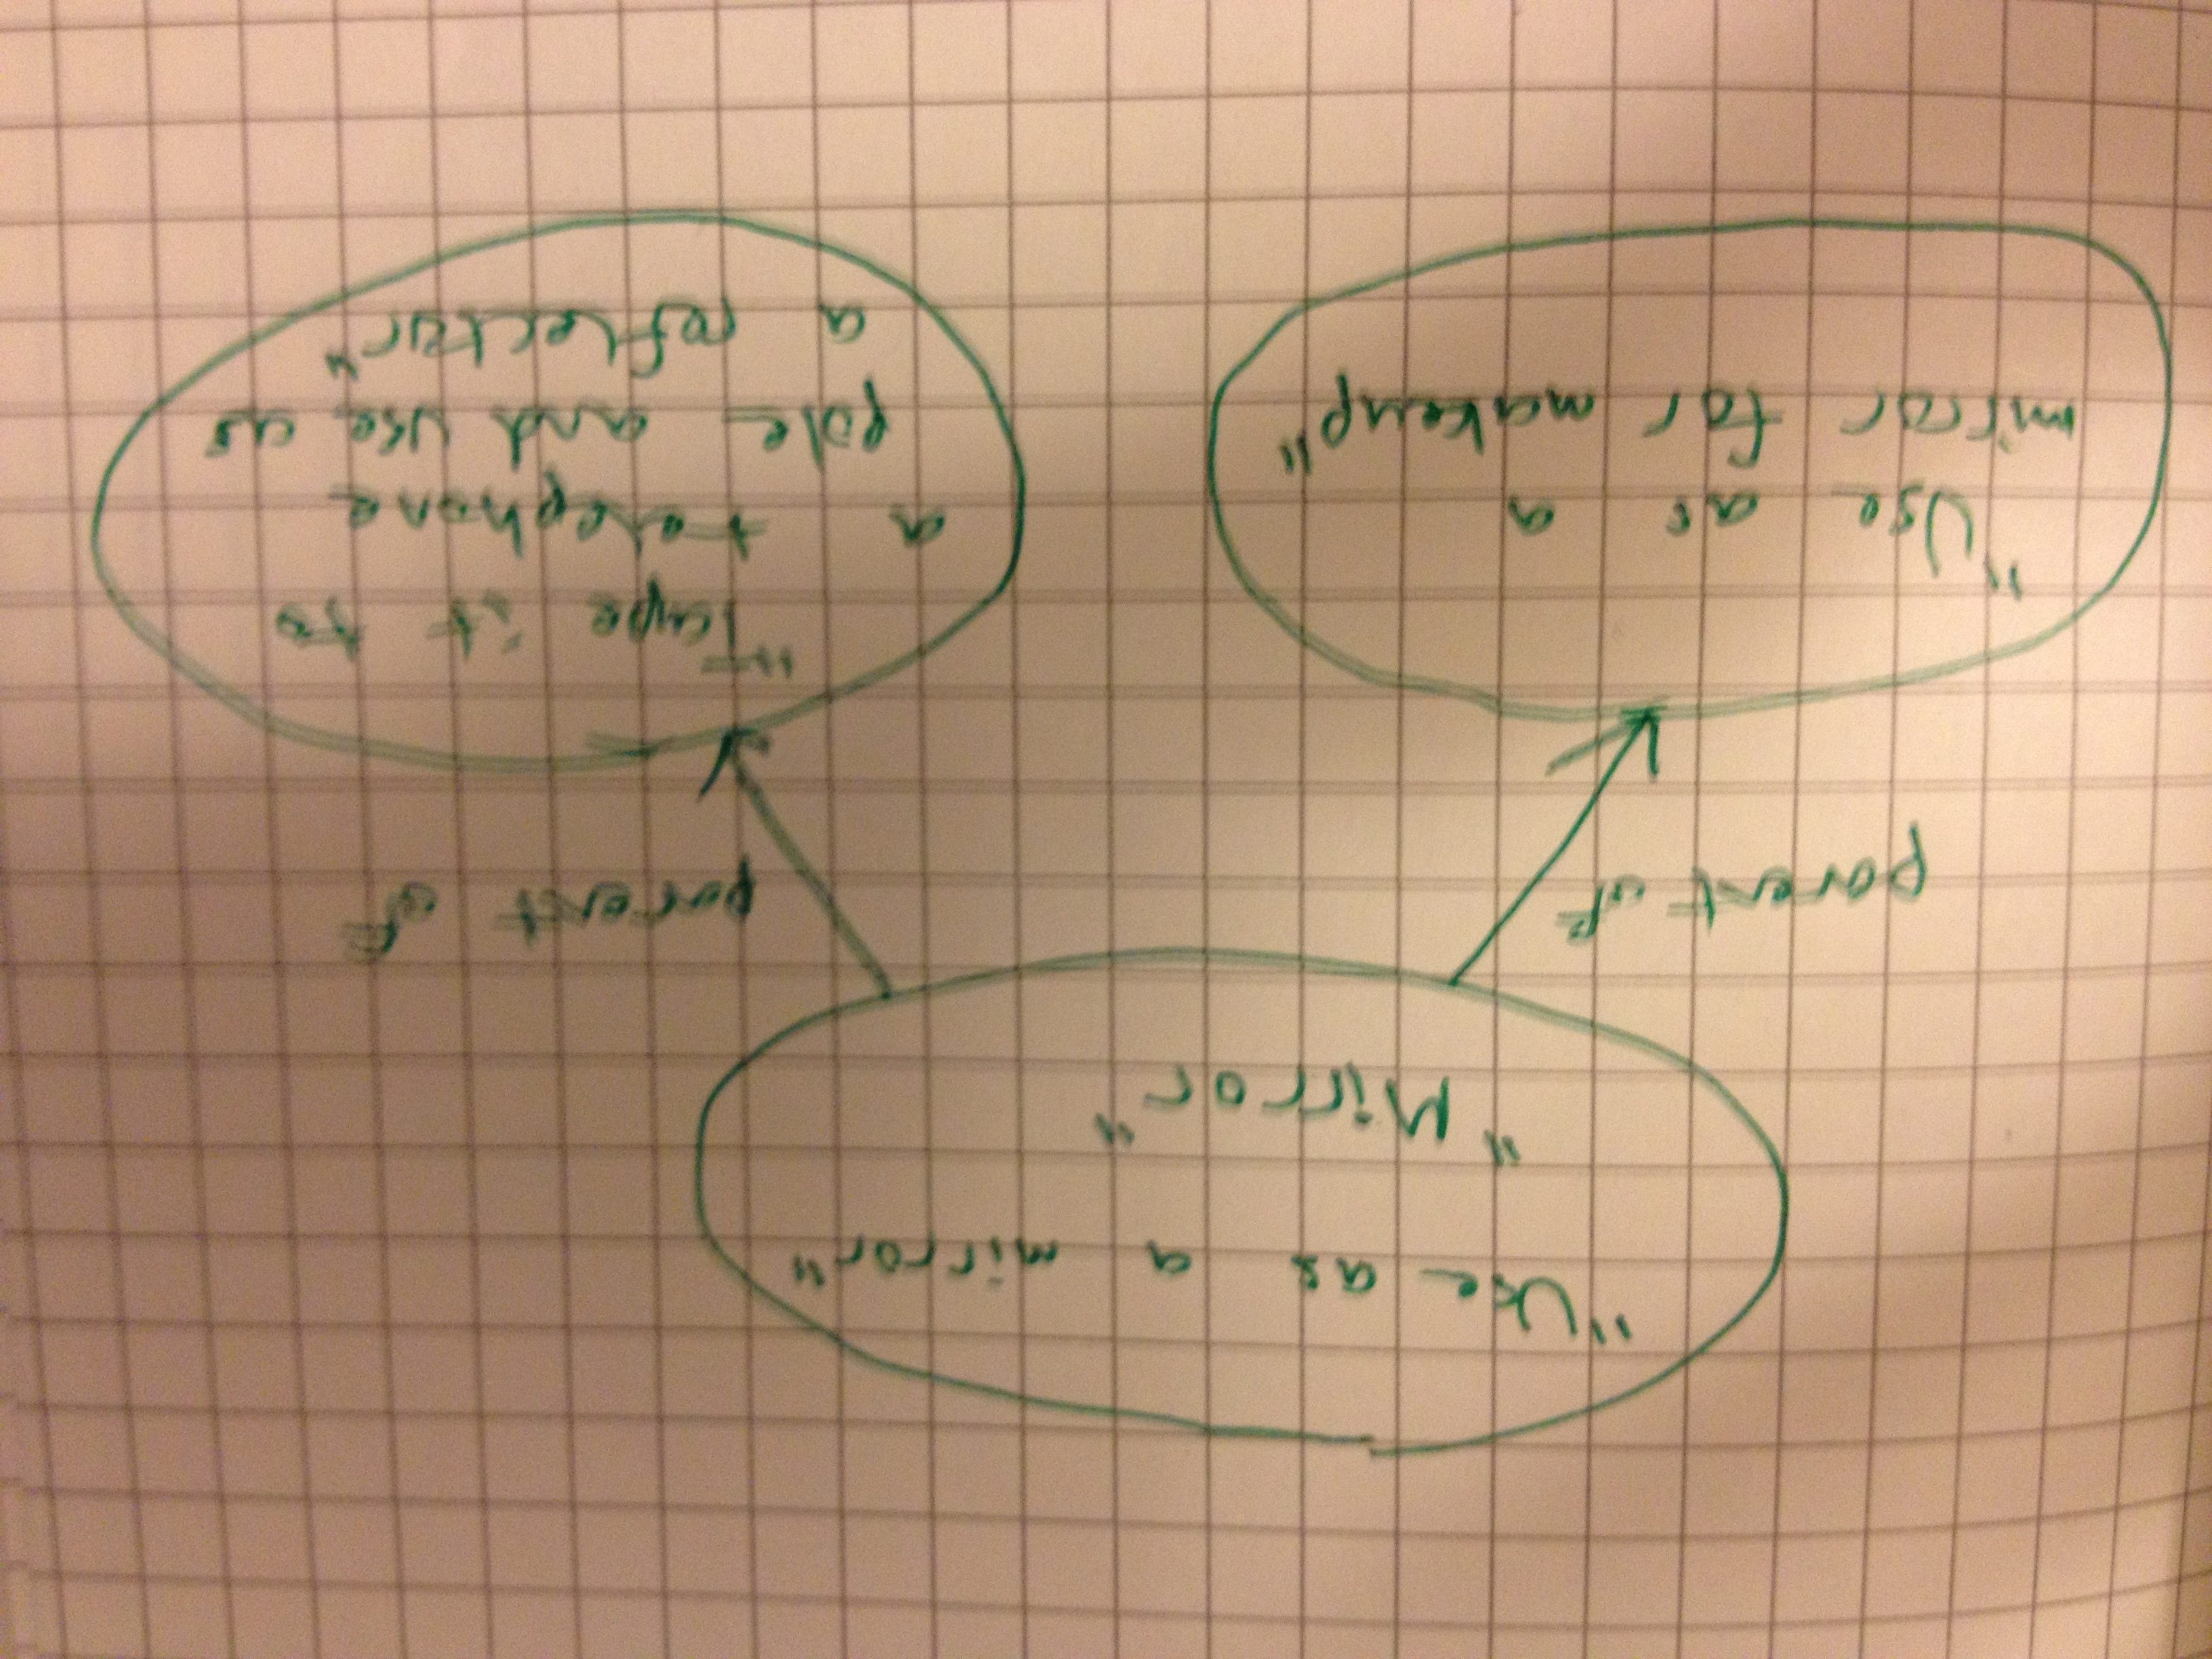
\includegraphics[width=0.9\columnwidth]{sample_category_tree}
\end{figure}

If an idea \emph{A} is a parent of idea \emph{B}, A is a generalization of B: all instances in A are are suitably general to encompass all instances in B. This difference is relative to the ideas in question.

A \emph{question forest} is simply the collection of all category trees generated in response to a particular question. Different trees in a question forest have no special relationship in meaning.

\subsection{Coding}

One researcher coded the data to produce the idea forests described above. The clustering algorithm is described in Figure FIG. Instances are added one at a time to the existing idea forest. In brief summary, the root idea that most closely matches the strategy in the instance is selected, and then that root idea and the new instance are compared in generality. This process may be repeated depending on this generality relationship, until instance is either placed in an existing idea or a new idea node is created.

The clustering algorithm relies on the human intelligence of the researcher for three key decisions:

\subsubsection{Similarity}
Two ndodes a and b have high similarity if they solve the problem in the same way, and low similarity if their solutions have no common themes. For example, in Figure FIG, "Mirror" and "Tape it to a telephone pole and use as a reflector" have high similarity, as they both solve the problem of using a broken MP3 player by using it to reflect light.

\subsubsection{Coverage}
A node a has high coverage of a node b if the problem solution in a is equal to or an abstraction of the problem solution in b. Coverage is not commutative. To return to the example, "Mirror" has high coverage of "Tape it to a telephone pole and use as a reflector", as the latter is a specific use for a mirror. On the other hand, the latter idea has low coverage of the former.

\subsubsection{Artificial Ideas}
Occasionally, two nodes have high similarity but no coverage. For example, "Use it as a mirror for makeup" and "Tape it to a telephone pole and use as a reflector" use the MP3 player in the same way, but neither is a generalization of the other. In this case, the algorithm appeals to the human coder to provide a lable for a new idea that is a generalization of both.

\begin{figure*}[h]
\begin{verbatim}
for each instance:
  idea_node = new node including instance
  current_node = root of forest
  do:
    best_match = max_similarity(idea_node, current_node.children)

    if best_match.similarity is low or current_node has no children:
      insert idea_node under current_node
      exit do
    else:
      if coverage(idea_node, best_match) == coverage(best_match, idea_node) == high:
        merge idea_node, best_match
        exit do
      else if coverage(idea_node, best_match) == coverage(best_match, idea_node) == low:
        new_parent = new artifical idea node
        insert best_match, idea_node under new_parent
        insert new_parent under current_node
        exit do
      else if coverage(idea_node, best_match) > coverage(best_match, idea_node):
        replace best_match with idea_node in tree
        current_node = idea_node
        idea_node = best_match
      else:
        current_node = best_match
\end{verbatim}
\caption{Manual clustering algorithm}
\label{fig:cluseringalg}
\end{figure*}

After completion of the coding algorithm, we were left with an idea forest as described in section SEC.


\section{Results}

We can use the uniqueness measure to understand the rate at which new ideas arrive. As we gather more and more ideas in the course of an experiment, we expect that we will see fewer ideas that are not already in our idea pool. Figure FIG shows the cumulative count of ideas as a function of the number of instances gathered in the experiment. To smooth the plot, the order in which instances were received was shuffled 100 times, and the mean of the cumulative unique idea count was taken at each step.

\begin{figure}[h!]
    \centering
    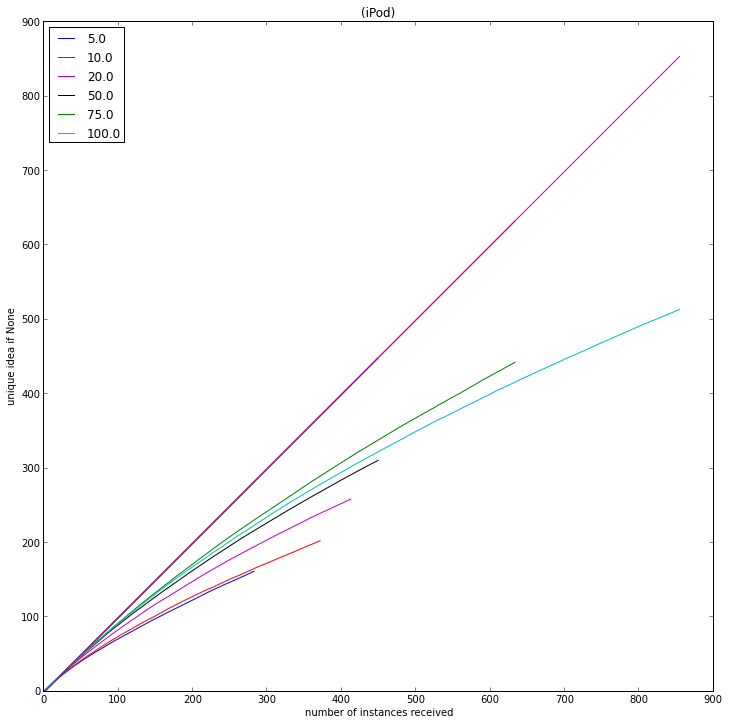
\includegraphics[width=0.9\columnwidth]{ideas_over_time}
    \caption{Cumulative idea count}
\end{figure}

The horizontal line in Figure FIG represent the idea case, in which each instance represents a different idea (i.e. every answer we receive is a new, unique idea). As expected, the rate at which ideas are gained appears to taper off.

Figure FIG more closely examines the rate, the primary property of interest. The panels, from top to bottom, are the rate at which new ideas, categories, and non-singleton categories are generated, respectively. Similar to Figure FIG, these are based on shuffling the order of instances 10000 times and taking the mean of the derivative at each point. In this case, the ideal (a 1:1:1 instance:idea:category ratio) is represented by the horizontal bar across the top of the chart.

\begin{figure}[h!]
    \centering
    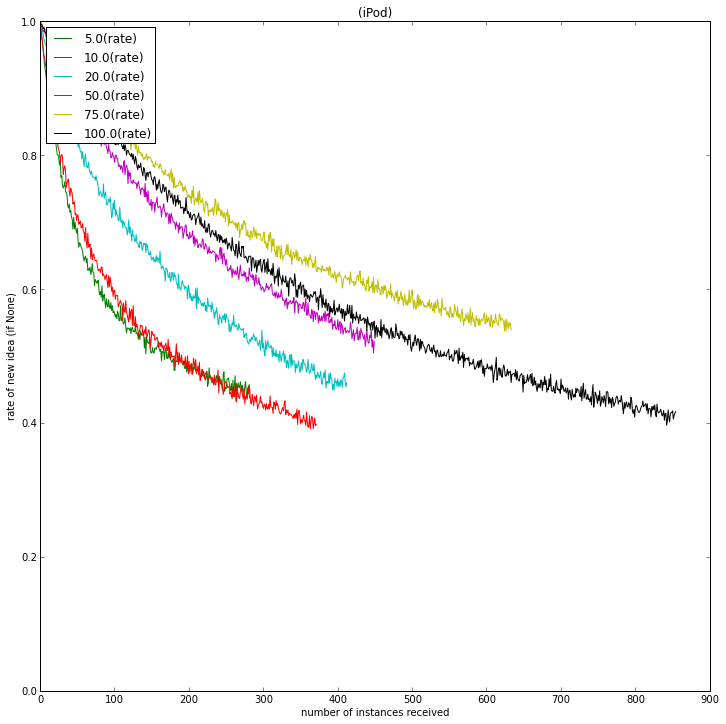
\includegraphics[width=0.7\columnwidth]{rate_new_idea_over_time}
    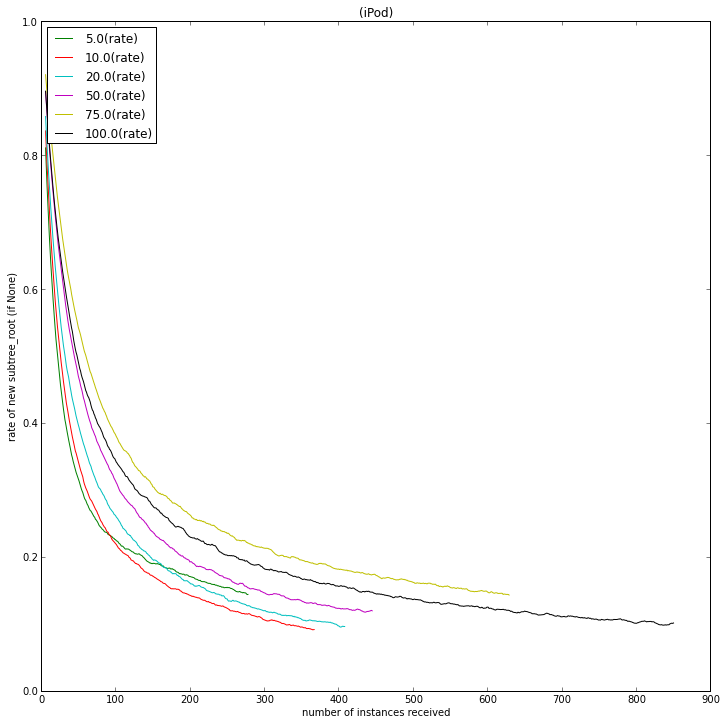
\includegraphics[width=0.7\columnwidth]{rate_new_category_over_time}
    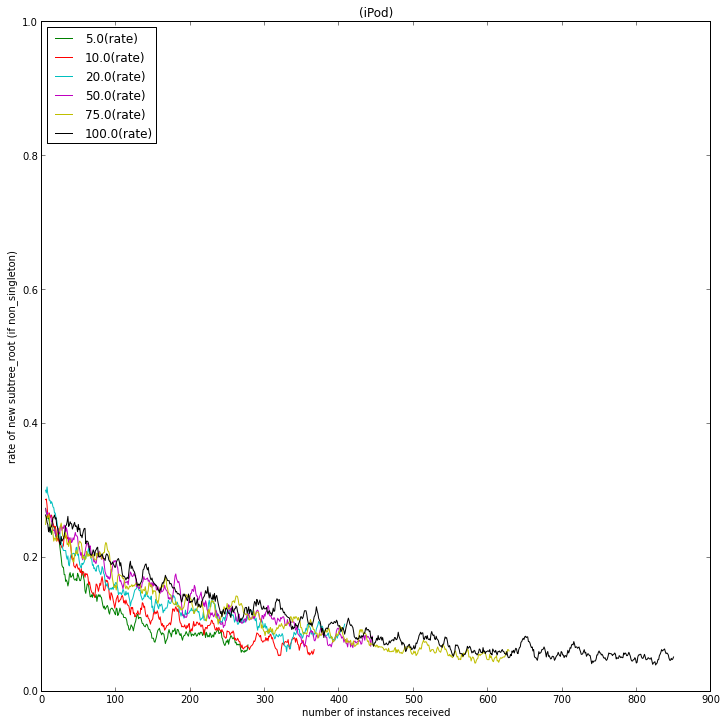
\includegraphics[width=0.7\columnwidth]{rate_new_ns_category_over_time}
    \caption{Rate of idea generation}
\end{figure}

The number of ideas, categories and non-singleton each drop off exponentially over time. It is unsurprising that the number of new categories should drop off faster than the number of new ideas, as we expect that there are fewer categories of ideas than there are individual ideas themselves.

The third panel, which shows non-singleton categories over time, tells a distinctly different story from the others. While in the idea and category plots, the height-ordering of rates of generation between categories remains generally identical, there is a point of intersection and reversal in the non-singleton category plot at around the 30 instances point. Before this point, the lower conditions actually generate new categories at a \emph{faster} rate.

In lower conditions, brainstormers will quickly offer up big, popular, non-singleton categories. Beyond the inflection point, the category pool is saturated with these low-hanging fruit, and only brainstormers tasked with generating more ideas will find the smaller category. This is a more nuanced view of the tree node/instance quartiles in Section SEC; condition 5 brainstormers cover the spectrum of category sizes while condition 100 brainstormers pull from the smaller category trees in the forest.

\subsubsection{Hypothesis 1}

Visually, the rate of idea, category and singleton category generation seems to trend towards 0. We tested this hypothesis...

Additionally Figure FIG indicates that there is some effect of number of ideas requested on the rate of generation. Generally, conditions with more requested responses generated ideas and categories at a higher rate.

Test here...

\subsubsection{Hypothesis 2}

Test here...

\subsection{Originality}

We measure differences in originality between conditions by examining the idea o-score and category o-score. The distributions of these scores are summarized in Figure FIG. The left panel compares idea o-score and the right compares category o-score.

\begin{figure}[h!]
    \centering
    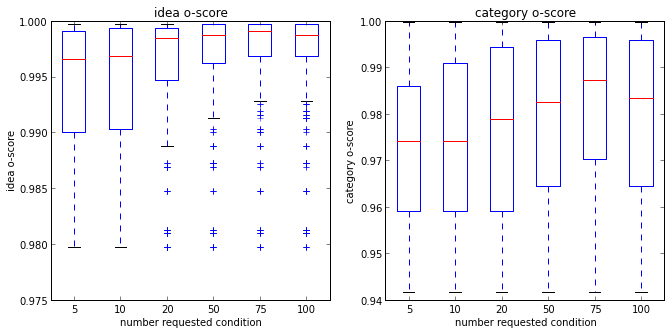
\includegraphics[width=0.9\columnwidth]{oscores_conditions}
\end{figure}

The more ideas requested, the more original the ideas produced. As suggested by the instance quartile range in section SEC, higher number conditions produce idea in trees with fewer instances, thus the high category o-score. We also see that these conditions produce \emph{ideas} with fewer instances.

As the originality rises, however, so does the number of outliers. To understand this phenomenon, we need to more closely observe the distribution of originality scores between not just conditions, but ordinal position in a brianstorming run.

Figure FIG provides this visualization. The upper panel gives the mean idea o-score as a function of ordinal position in all 100 condition brainstorming runs. The o-score for each ordinal position is the mean of all idea o-scores for that ordinal position in a run. Following this, the plot is further smoothed by making each point the mean of a sliding window of size 10 around its ordinal position. The bottom panel is a similar plot for category-oscore. To aid in interpretation, the first, second and third quartiles are also represented on the plot. The error bars are standard error.

\begin{figure}[h]
    \centering
    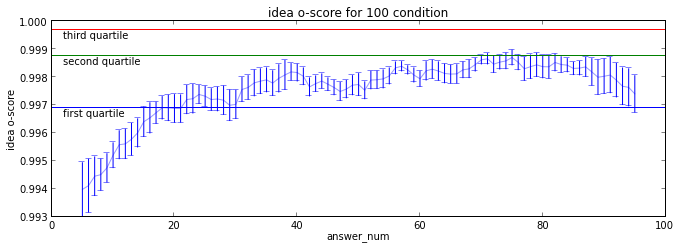
\includegraphics[width=0.9\columnwidth]{idea_oscore_order_100}
    \caption{Idea o-score as a function of order (100 condition)}
    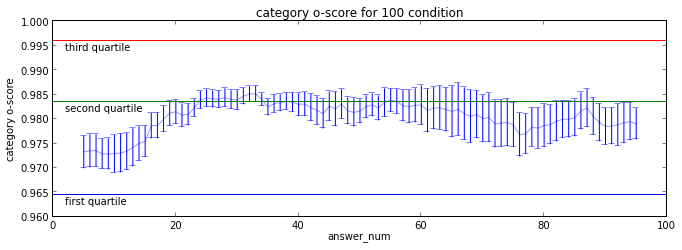
\includegraphics[width=0.9\columnwidth]{cat_oscore_order_100}
    \caption{Category o-score as a function of order (100 condition)}
\end{figure}

The only part of the originality score that falls outside the first and third quartiles is the beginning of the run. Participants in the higher numbered conditions generate more original ideas overall, but not until they have exceeded some threshold of common ideas. Figure FIG replicates figure FIG but across all conditions, and the same pattern of originality growth until an originality peak - around 20 ideas - is reached. Note that because of the additional HITs, there are far more examples of early-order ideas in the 5, 10 and 20 conditions than in the 50, 75, or 100, so this pattern is present without any dominating affect by the upper conditions.

\begin{figure}[h]
    \centering
    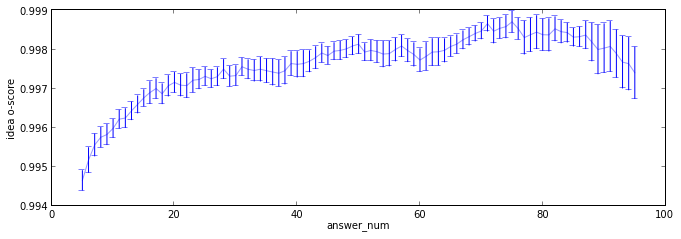
\includegraphics[width=0.9\columnwidth]{idea_oscore_order}
    \caption{Idea o-score as a function of order}
    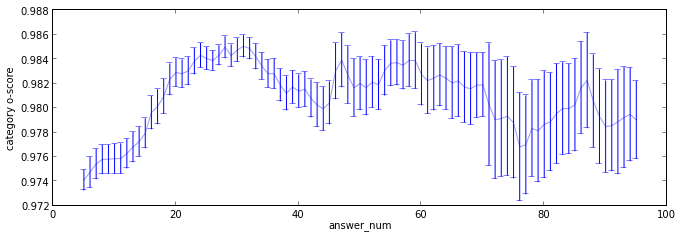
\includegraphics[width=0.9\columnwidth]{cat_oscore_order}
    \caption{Category o-score as a function of order}
\end{figure}

A similar, although less severe, pattern is observed for category o-score. There is a gradual increase in category originality until the 20 instance threshold is reached, at which point variance of the scores increases rapidly and no clear pattern is observable. This is explained by the relationship between common ideas and common categories. We expect that unoriginal ideas belong to unoriginal categories, as a high instance count for an idea increases the instance count for its category tree. However, we cannot make the inverse assumption, that a high originality idea belongs to a high originality category. Once the common idea are exhausted, then, there is no relationship between idea originality and category originality.

\subsubsection{Hypothesis 3}

This interpretation supports \textbf{Hypothesis 3:} There is a set of general, common ideas that make up the first several responses of every crowd brainstorming session, regardless of condition. We test this interpretation by constructing a set of the top 66 (5\%) most common ideas. If our intuition is correct, these ideas should be more likely to appear in the first 5 instances of a run than they are to appear in any of the following instances. We designate two Bernoulli variables. The first, defined by parameter $\theta_f$, represents the probability that an instance is in the common set given it is in the first five instances of a run. The second, defined by parameter $\theta_l$, is the probability that an instance is in the common pool given it is one of the \emph{last} (>5) instances in a run..

We fit these parameters using data from all runs with a total number of instances greater than 10. We chose this so that no run could contribute evidence to $\theta_f$ without also contributing to $\theta_l$. The resulting parameters were $\theta_f = 0.564$ (95\% HDI 0.517-0.611) and $\theta_l = 0.323$ (95\% HDI 0.303-0.342). This difference is significant, supporing the hypothesis that common ideas are over-represented in the early part of a brainstorming run, regardless of conditon.


\subsubsection{Hypothesis 6}

This threshold at 20 ideas brings us to \textbf{Hypothesis 6:} Ideas generated in the latter half of a brainstorming session are of higher originality than ideas generated in the former half. With our empirical evidence, we can instead test that ideas \emph{more than 20 instances into a brainstorming session} are more original than those in the first 20 instances, regardless of condition.

Test here...

\subsection{Riffing: We need to change the name of this}

At the level of the individual brainstorming run, we examine a new phenomenon related to uniqueness above. Within the SIAM model, \emph{riffing} (or \emph{clustering} as it is known in the work) occurs when a single participant activates a single image (analogous to a non-singleton category) and produces multiple ideas from that image under a fail state is reached and a transition is undergone to a new image. Unsurprisingly, we observed riffing activity in our data. An example of a single participant's riffed responses is given in Figure FIG. The second column is dark if the instance is a \emph{look-back equal} to any idea earlier in the run. The first column is dark if the instance is a \emph{source} instance, meaning it is the first in a chain of look-back equal instances. Riff chains can either be consecutive (as in the example), or separated with instances in between. The third column simply provides the text for that instance.

\begin{figure}[h]
    \centering
    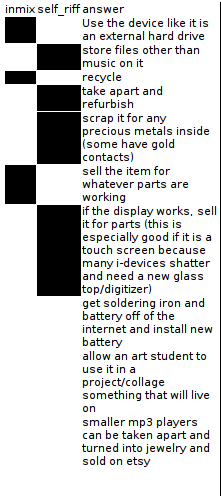
\includegraphics[width=0.5\columnwidth]{10_riff}
    \caption{Example of riffing in a size 10 run}
\end{figure}

The participant hits on the categories of using the device's hard drive for storage, recycling the device or its materials, and selling the device.  within these categories, they generate 2-3 ideas each. This is a fairly typical example of riffing. In larger conditions, it is common for participants to reach further back and return to an idea multiple time. Table TAB provides a summary of riffing between conditions.

\begin{table}
\begin{tabular}[h!]{r | l l l l l l l}
    \hline \hline \textbf{condition} & 5 & 10 & 20  \\ \hline \hline
    \% riffs & 13.65 & 19.28 & 25.17  \\
    source instances & 10.58 & 12.92 & 15.01 \\
    riffs per source & 1.29 & 1.49 & 1.68 \\
    median length of consecutive chain & 2 & 2 & 2 \\
    median distance to previous in chain & 1 & 2 & 2 \\
    median distance to first in chain & 2 & 3 & 5 \\ \hline \hline
    \textbf{condition} & 50 & 75 & 100 \\ \hline \hline
    \% riffs & 39.6 & 32.81 & 42.81 \\
    source instances & 19 & 17.19 & 18.13\\
    riffs per source & 2.08 & 1.91 & 2.36\\
    median length of consecutive chain & 2 & 2 & 2\\
    median distance to previous in chain & 7 & 10 & 5\\
    median distance to first in chain & 16.5 & 18 & 26.5 \\
    \end{tabular}
    \caption{Riffing statistics by condition}
\end{table}

The higher the number of instances requested, the more participants riff on their old ideas. Similarly, upper conditions use more of their ideas as sources for riffing, and riff more times on each of those ideas. The primary surprise is that they do not riff more consecutively. The median length of a consecutive riff chain remains low across conditions. This leaves us with the image of a participant in the upper conditions searching through their old ideas for something to build upon one instance at a time.

Another outlier of note is the relatively short median distance to a previous idea in a chain for the 100 condition. Participants in the 100 condition may feel more pressure to remix, and return to earlier ideas more quickly than those in the 50 or 75 conditions.

\subsubsection{Hypothesis 4}

Riffing activity is analogous to idea production within an image as described by Nijstad and Stroebe's SIAM model \cite{nijstad_how_2006}. Thus, we should expect to confirm their hypothesis, \textbf{Hypothesis 4}, that \emph{an idea from one semantic category should more often by followed by an idea from the same category than expected by random chance}.

To test this, we modelled the probability of any category being followed by the same category with a Bernoulli distribution. Each instance not the first in its run was a trial. If the instance was in the same category tree as the previous instance, the trial was a pass. Otherwise, it was a failure. The Bernoulli $\theta$ was 0.156 (95\% HDI 0.143 - 0.170).

The most common category tree in our data set, \emph{music player}, represents only 5.65\% of instances. This is well below the 0.143 lower-bound of HDI. Thus, we accept the hypothesis that an instance follows a previous instance in the same category with greater probability than is explained by random chance.

\subsection{Completion Time}

As another aspect of how participants complete brainstorming runs, we are interested in the time spent on each response. The first, second and third quartiles for each condition are given in boxplots in figure FIG. The whiskers extend to 1.5 times the inner quartile range. Surprisingly, we see many instances taking up to 28018382ms (7.78 hours) to complete.

\begin{figure}[h]
    \centering
    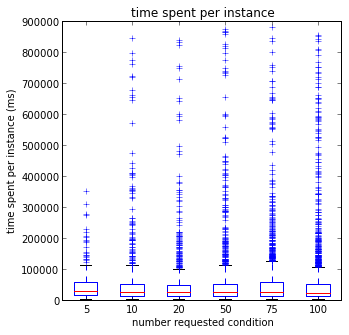
\includegraphics[width=0.9\columnwidth]{time_spent_condition}
    \caption{Time spent per instance}
\end{figure}

Either our participants were exceedingly concerned with crafting their responses, or there is another influence at work. Figure FIG gives the mean time spent on an instance by order, separated by condition. Most of the highly variant response times take place early in the brainstorming run. This suggests that at least one participant accepted a brainstorming task, took an initial stab at instances, and then left the task for up to 8 hours before continuing. Beyond this, we might expect to see time spent per instance go up as participants have to dig deeper to find responses, but no such effect is consistently observed.

\begin{figure}[h]
    \centering
    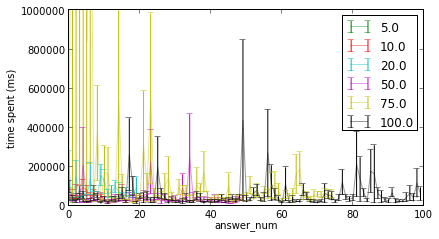
\includegraphics[width=0.9\columnwidth]{time_spent_order}
    \caption{Time spent per instance}
\end{figure}

\subsubsection{Hypotheses 5}

The Nijstad and Stroede \cite{nijstad_how_2006} model also provides \textbf{Hypothesis 5}: \emph{idea generation when changing semantic categories should take longer than idea generation within categories}. An examination of the distribution of data for time spent per instance suggested a log-normal distribution, with the frequency of occurances quickly rising until a peak was reached, followed by a gradual drop-off. As with previous tests, we used the Stan package for Bayesian inference [CITE]. We fit, two models: $t_w = \text{lognormal}(\mu_w, \sigma_w)$ for within-category idea generation and $t_b = \text{lognormal}(\mu_b, \sigma_b)$ for between-category idea generation, where the $t$ parameter in each model represents the time spent generating an instance.

\begin{figure}[h]
    \centering
    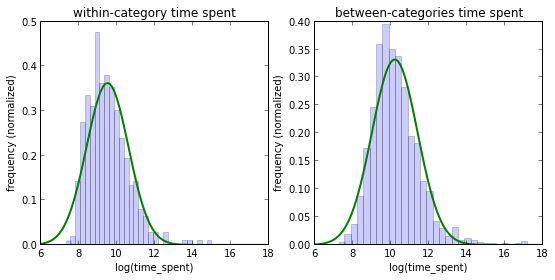
\includegraphics[width=0.9\columnwidth]{hyp5_comparison}
    \caption{Time spent to generate an instance}
\end{figure}

The resulting fit models are shown in Figure FIG, overlapping the log-space histograms for observed values. The mean for the within-category condition was 9.5 in log space (13.4 seconds, 95\% HDI 9.4-9.6), while the mean for the between-categories condition was 10.2 (27.0 seconds, 95\% HDI 10.2-10.3). The variances were 1.1 (3 seconds) and 1.2 (3.3 seconds) respectively. These difference were both sigificant. Within-category instance generation took on average 12.6 seconds less than between-categories. This is consistent with the findings of Nijstad and Stoebe, who reported differences of 6-12 seconds.


%\section{Qualitative analysis}


We selected 30 brainstorming runs (5 randomly from each condition). The primary author applied an open coding strategy, identifying \emph{strategies}: plans or rules that aid in generating ideas. We describe the observed strategies in detail below.
We describe the distribution of these strategies across runs and comment on variability between participants.

\subsection{Strategies}

A \emph{strategy} is a plan or rule, that is used by a participant to generate brainstorming responses. We infer the existence of strategies through similar classes of ideas observed between participants.
We identified 3 strategy categories, each of which can be employed with or without any of the other categories.
The first, \emph{problem scoping}, is a process in which a participant chooses a limited implication or component of the problem and provides multiple solutions.
The second category expands on the \emph{riffing} phenomenon introduced earlier.
%Finally, the \emph{humour} strategy emphasizes generating ideas that are amusing rather than practical.
Finally, the \emph{partial solution} strategy entails creating an idea that requires further idea generation to solve the problem.

\subsubsection{Problem scoping}

Under the problem scoping strategy, the original problem is transformed to a new problem of reduced scope.
Many transformations of the MP3 problem are possible, for example: brainstorm uses for \emph{an audio output device}; brainstorm uses for \emph{a hard drive}; and so on. The participant chooses a problem transformation and generates solutions, each of which is also a solution to the original problem. For example (PXXX):

\begin{itemize}
    \item have them as a resource on public transportation -- people must supply their own headphones
    \item use them in museums to give information on various installations
    %\item have cities install them in tourist areas, so people can listen about where they are
\end{itemize}

The participant's responses satisfy the transformed question "brainstorm uses for an audio output device". Resulting ideas no not rely on other aspects of the problem.

We distinguish between two types of problem scoping. \emph{Inward scoping} transformations reduce scope by limiting consideration to a single detail of the problem. The previous responses, which focus on audio output, are an example of inward scoping.

\emph{Outward scoping} transformations reduce complexity by stripping meaningful details. For example (PXXX):

\begin{itemize}
    \item doorstop
    \item use in abstract art
\end{itemize}

These solutions could be applied to a wide body of problems unrelated to the original, such as "brainstorm uses for a broom".
In contrast, inward scoping solutions are applicable to the transformed problem and the original problem, but not many others. Thus, a useful rule for distinguishing the types of scoping is to consider whether the \emph{set of problems solved by the solutions} is small, or large.

Some responses employ no scoping whatsoever. These responses utilize the device exactly as it was intended, as a portable MP3 player. For example, "get it fixed and give it to a needy kid" (PXXX).

\subsubsection{Riffing}

The second category of strategies is \emph{riffing}.
We found riffing manifested itself many ways, and identified four distinct riffing strategies used by participants: generalization riffing, repeat riffing, hold riffing, and continuation riffing. 

\emph{Generalization riffing} occurs when a participant generates two or more ideas and one is a generalization of the other. For example, two consecutive ideas given by PXXX:

\begin{itemize}
    \item brick
    \item building material
\end{itemize}

Another type of riffing is \emph{repeat riffing}. Under this strategy, a participant produces multiple responses, such that the group of ideas could be easily summarized as one idea without significant loss of information. For example (PXXX):

\begin{itemize}
    \item extract usage data
    \item extract texts
    \item extract gps data
\end{itemize}

In this case, all three ideas could be summarized with "extract the data on the device".

\emph{Hold riffing} is a strategy in which participants hold at least one element of a previous response constant when generating a new response. For example (PXXX):

\begin{itemize}
    \item Jukebox music selector in bars
    \item Commercials in bar bathrooms 
    \item Tapper handles for beer 
\end{itemize}

In this example, the setting of the application is held constant across riffs: a bar.

Another realization of hold riffing holds language term constant between unrelated ideas. For example (PXXX):

\begin{itemize}
    \item We could use the hard-drives inside for different electronics.
    \item We could use them in place of rocks (to throw at things, to use in pavement.)
\end{itemize}

\emph{Continuation riffing} is the strategy of creating another idea that cannot be understood without the context of the previous. For example (PXXX):

\begin{itemize}
    \item I suppose you could just grind them down into a sand
    \item You could take the sand... and put it in an hourglass
\end{itemize}

\paragraph{Spatial separation}

%The strategies above describe techniques for taking one idea and transforming it into another.
In this section, we describe patterns of \emph{where} participants implemented strategies.

The most natural separation between a riffed idea and its source is none - the riffed idea directly follows the source. We call this \emph{linear riffing}.
\emph{Reach backs} entail riffing on an idea that occurred further back in the run than the previous response. 

Finally, some participants \emph{pair} their riffs. Paired riffing is a special case on linear riffing in which only a single riffed idea is produced. For example, paired repeat riffing from PXXX:

\begin{itemize}
\item cut up and use to decorate shoes
\item cut up and use to decorate vase
\end{itemize}


\subsubsection{Partial solutions}

Under this category of strategies, responses provide some elements of a solution to the problem, but further idea generation is required to implement the solution. The following ideas (PXXX) are all examples of partial solutions:

\begin{itemize}
    \item use old parts to make a new device
    \item old parts can use to make something
    %\item create a new device
\end{itemize}

In these responses, there is a recommendation that we produce new electronics, but it is unclear what we would make. 

There are four sub-strategies of partial solutions: problem scoping without solution, goal without plan, plan without goal, and passing the problem. 

In some responses, an end goal has been established, but executing the goal requires additional information. We call this strategy \emph{goal without plan}. The above responses are examples of the goal without plan strategy.

The inverse of this strategy is \emph{plan without goal}, as demonstrated in these responses (also from PXXX):
\begin{itemize}
    \item melt down old parts
    \item see what old parts are usable
\end{itemize}
In this case, the operations of melting down the device or checking for working parts can be performed, but don't provide any obvious benefit.

Responses that do not have an explicit goal or plan may nonetheless imply one. For example, "throw it in the ocean" (PXXX) has the implied goal of disposing of the broken device. In these cases, responses do not employ a partial solution strategy.

Above, we described the problem scoping strategy. Some participants performed \emph{problem scoping without solution}, in which problem scoping is the only component of the response.
For example (PXXX): "Remove glass screen to make something". In this case, the participant has provided a scoping of the problem (focus on the glass component) but has not actually provided a solution to the scoped problem.

Finally, responses in the \emph{pass the problem} strategy relocate the need for idea generation to a third party. These responses from PXXX provide an example:

\begin{itemize}
    \item give to non-profit that can benefit
    \item give to an organization that has the knowledge to use these devices
\end{itemize}

In this case, a third party must determine what to do with broken MP3 players.

\subsection{Strategy use}

In this section, we DESCRIBE how strategies were employed by participants. The primary author again coded 30 randomly selected runs (5 from each condition, 1150 instances total) for the strategies identified above. Note that examples of riffing identified in this section are distinct from the category tree identification of riffing described in the method section above. The prevalence of each strategy is given in Figure FIG.

%\begin{table}
%    \begin{tabular}{r | l l}
%        \textbf{strategy} & \textbf{\# instances} & \textbf{\% of instances} \\
%        inward scoping & 267 & 23.2 \\
%        outward scoping & 828 & 72 \\
%        no scoping & 55 & 4.8 \\
%        \hline \hline
%        hold riffing & 278 & 24.2 \\
%        continuation riffing & 3 & 0.3 \\
%        repeat riffing & 119 & 10.3 \\
%        generalization riffing & 48 & 4.2 \\
%        \hline
%        any riffing & 448 & 39.0 \\
%        pair & 108 & 9.4 \\
%        reach back & 129 & 11.2 \\
%        \hline \hline
%        scoping without solution & 3 & 0.3 \\
%        passing the problem & 69 & 6 \\
%        plan without goal & 58 & 5.0 \\
%        goal without plan & 58 & 5.0 \\ 
%        \hline
%        any partial solution & 188 & 16.3 \\
%    \end{tabular}
%\end{table}

\begin{figure}[h!]
    \centering
    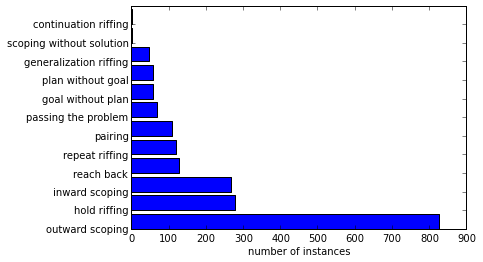
\includegraphics[width=0.9\columnwidth]{strategy_counts}
    \caption{presence of strategies}
    \label{fig:strategy_counts}
\end{figure}

Outward scoping is by far the most common strategy, occurring in 72\% of instances. Riffing is also very common, with 40\% of instances employing some form of riffing. Riffs are most often consecutive (linear riffing), and hold riffing is the most common type.

Partial solutions are fairly uncommon (16.3\%), and most often involve passing the problem (6\%). Continuation riffing and scoping without solution are the least common strategies, each with only 3 instances.

\subsubsection{Strategy location}

We also consider where in a brainstorming run the strategies are more likely to occur. The results are summarized in Table TAB.

\begin{table}
    \begin{tabular}{r | l l l l l l}
        \textbf{strategy} & \textbf{5} & \textbf{10} & \textbf{25} & \textbf{50} & \textbf{75} & \textbf{100} \\
        inward scoping & 2 & 5 & 11 & 23 & 29 & 44 \\
        outward scoping & 3 & 3 & 8.5 & 27.5 & 39.5 & 41 \\
        no scoping & 3 & 5 & 9 & 18 & 22.5 & 20.5 \\
        \hline \hline
        hold riffing & 3 & 8 & 12.5 & 24 & 44.5 & 57.5 \\
        continuation riffing & - & - & 18 & 4 & 27 & - \\
        repeat riffing & 4 & 7 & 2 & 25 & 49.5 & 45 \\
        generalization riffing & 4 & 4 & 11 & 29.5 & 34 & 30 \\
        \hline
        pair & 3.5 & 7.5 & 12.5 & 25.5 & 40 & 33.5 \\
        reach back & 3.5 & 6 & 11 &29.5 & 40 & 47.5 \\
        \hline \hline
        scoping without solution & - & - & - & 13 & - & 53 \\
        passing the problem & 1.5 & - & 14.5 & 40 & 35.5 & 60.5  \\
        plan without goal & - & - & 6 & 18 & 38.5 & 30 \\
        goal without plan & - & 3 & 2 & 15 & 11 & 29 \\ 
    \end{tabular}
    \caption{Median position of strategy in run by condition}
\end{table}

The distributions of strategy occurence across position in run tend towards uniform. The notable exceptions are problem scoping and reach-backs. There are fewer occurences of the inward scoping strategy later in brainstorming runs.
The number of reach-backs increase with position. 

%\subsubsection{Strategy co-occurrence}

%Of final interest was the question of which strategies occurred together. For each run, a count was taken of the number of occurrences of each strategy, and the Pearson r of these counts was taken for each pairing of strategies to give a rough measure of how the strategies were grouped in runs. Strong correlations (greater than 0.6) are given in Table TAB.

%\begin{table}
%    \begin{tabular}{l l l}
%        \textbf{strategy 1} & \textbf{strategy 2} & \textbf{Pearson r} \\
%        \hline
%        passing the problem & repeat riffing & 0.89 \\
%        hold riffing & outward scoping & 0.85 \\
%        pairing & scoping without solution & 0.64 \\
%        reaching back & hold riffing & 0.64 \\
%        pairing & outward scoping & 0.63 \\
%        reaching back & outward scoping & 0.62 \\
%        plan without goal & hold riffing & 0.61 \\
%    \end{tabular}
%\end{table}

%Passing the problem and repeat riffing were highly correlated (0.89), indicating that responses utilizing pass the problem were likely to be repeated many times to generate more responses. For each of the other correlations, the potential implications less obvious. Further analysis is required to tease out the implications of strategy co-occurrence.

\subsection{Variability of Worker Input}
While we observed that individuals are likely to draw from a common pool of ideas early on in the brainstorming process, there were outliers in the data. For example, one individual in the 75 ideas condition consistently produced some of most original ideas for old MP3 players:

\begin{itemize}
\item With displays - could be attached to a small solar panel (like the USB chargers w/multi attachments, including solar and car, etc.) and all the power could be sent to the screen as a small, portable light, then sent to countries lacking power in rural areas.
\item They could be loaded with coordinates or other info and sealed in containers, then used in ocean current studies - once the container was collected they could be plugged in and read, and the data could be sent to whomever.
%\item They could be plugged in at a base camp at the bottom of Everest, and then potential climbers could record their name, loved ones' address, and any last words before attempting the climb. 
\end{itemize}

This individual's responses raised the observed uniqueness of ideas in the 75 condition. 
In contrast, other individuals filled their quotas with excessive repeat riffing chains. 

This variability in worker responses prevented us from modeling any potential effects that the number of questions requested might have on individuals' responses. Thus, while it is clear that there is little advantage to requesting 5 or 10 ideas from workers, it is not clear whether it is preferable to request 20, 50, 75, or 100 ideas. We suspect that requesting 50 or 75 is the ``sweet'' spot, but are not able to empirically support that recommendation at this time.




\section{Discussion and Future Work}

In this paper, we have primarily focused on the uniqueness of ideas and idea categories in quantitative terms. In this section, we provide a more qualitative perspective on the data collected, then describe future work.

\subsection{Variability of Worker Input}
While we observed that individuals are likely to draw from a common pool of ideas early on in the brainstorming process, there were outliers in the data. For example, one individual in the 75 ideas condition consistently produced some of most original ideas for old MP3 players:

\begin{itemize}
\item With displays - could be attached to a small solar panel (like the USB chargers w/multi attachments, including solar and car, etc.) and all the power could be sent to the screen as a small, portable light, then sent to countries lacking power in rural areas.
\item They could be loaded with coordinates or other info and sealed in containers, then used in ocean current studies - once the container was collected they could be plugged in and read, and the data could be sent to whomever.
\item They could be plugged in at a base camp at the bottom of Everest, and then potential climbers could record their name, loved ones' address, and any last words before attempting the climb. 
\end{itemize}

This individual's responses were responsible for clearly raising the observed uniqueness of ideas in the 75 condition when plotted against the other conditions.

Other individuals filled their quotas by creating uninspiring idea templates that they varied only slightly between responses. For example:

\begin{itemize}
\end{itemize}

\subsection{Future Work}
The most immediate work that follows from this is to examine the same phenomena for multiple questions. A design space for brainstorming taks must be defined and tested to see how variations impact the rate of idea generation, originality, etc.

The saturation point of unique ideas and categories presents an obstacle to large-scale brainstorming on microtask marketplaces. One could conceivable develop interventions to overcome and reset this stagnation behaviour. For example, ideas from previous responders could be interspersed in response fields of the task to promote riffing or combination.

We identified that ideas are more likely to be followed by one from the same category, and that changing categories takes time. Combining these models with others (such a natural language measures for text similarity), one could construct a posterior belief model for whether a participant is currently riffing.

The change in idea and category o-scores at the 20 instance point is reflected in other metrics not discussed in this paper. It is likely this represents a distinct strategy change. By modelling this strategy change explicitly, we may be able to identify more explicitly when this change happens and make predictions about later strategies based on those employed early in the brainstorming run.




\subsection{Implications}

From these, we draw several implications. First, that there is a saturation point in number of unique ideas or idea categories received, beyond which results will stagnate.

anyone seeking creative brainstorming results in microtask environments should ask for more than 20 ideas per participant.

Although idea o-score goes up over time, category o-score increases and then reaches a point of high variability. This implies a change in the strategy of how categories are used. It may be that beyond 20 ideas, high idea o-scores are maintained via a mix of remixing within existing categories (low category o-score) and establishing entirely new images (high category o-score).



%We set out to establish a baseline for brainstorming performance in crowd marketplaces, a new setting for idea generation in with spatial and temporal co-presence are not guaranteed. We did this by establishing a corpus of brainstorming responses, publically available at URL. Furthermore, we introduce the \emph{idea forest}, an encoding of brainstorming responses that captures differences in generality we discovered, an introduced an algorithm for producing idea forests.

%We found that originality increased as brainstorming participants were asked to generate more ideas individually. Generality, however, decreased. In both cases, we found a ``sweet spot" for this change at the 20 idea mark; participants' ideas reach their peak creativity and minimum generality after their 20th contribution.

%Furthermore, we verified that the findings and predictions of prior work in which participants were spatially and temporally copresent. We found that, in line with the predictions of Jigstad and Stroebe's SIAM model \cite{nijstad_how_2006}, ideas are more likely to follow an idea of the same category than would be randomly expected, and that the time spent to generate an idea within-category is lesser than that to generate ideas between categories. Furthermore, we recreated the finding of Parnes et al \cite{parnes_effects_1961} that responses in the latter part of a participant's idea generation process are more creative than those earlier.

%We identified three qualitative phenomena in of brainstorming results. First, that brainstorming results are subject to the popular consciousness of the time they are gathered. Second, that workers are more likely to take HITs with higher absolute payout, even if relative payout is identical.

%The most salient recommendation we can make is easily summarized: if you use the crowd for brainstorming and desire originality, it is most productive to ask few participants for more than 20 ideas each.

\section{Conclusion}

In this work, we developed models of idea generation, category geneartion, originality, and individual practice in brainstorming on microtask markets.
These models provide a baseline for both structure and performance in this context. They allow us to provide recommendations for idea solicitors, and starting points and comparison statistics for researchers.

 We summarize our findings:

\begin{itemize}
\item The rate of idea and category generation decays non-linearly over time. 
\item Common ideas are more likely to be proposed early in a run. 
\item Conversely, ideas beyond the first 20 are rarer and more original, as measured by o-scores. This relationship also holds for idea categories.
\item Ideas are more likely to be followed by another idea from the same category than would be expected by random chance.
\item The time it takes to generate an idea when changing categories is longer than the time when generating within a category.
\end{itemize}


\section{Future Work}

\subsection{Interventions}

\begin{itemize}
\item multi-phase brainstorming: introducing common ideas first to force workers more quickly into the originality zone
\end{itemize}

\subsection{Predicting Turker performance}

\subsection{Automatic Idea Forest Generation}


% Balancing columns in a ref list is a bit of a pain because you
% either use a hack like flushend or balance, or manually insert
% a column break.  http://www.tex.ac.uk/cgi-bin/texfaq2html?label=balance
% multicols doesn't work because we're already in two-column mode,
% and flushend isn't awesome, so I choose balance.  See this
% for more info: http://cs.brown.edu/system/software/latex/doc/balance.pdf
%
% Note that in a perfect world balance wants to be in the first
% column of the last page.
%
% If balance doesn't work for you, you can remove that and
% hard-code a column break into the bbl file right before you
% submit:
%
% http://stackoverflow.com/questions/2149854/how-to-manually-equalize-columns-
% in-an-ieee-paper-if-using-bibtex
%
% Or, just remove \balance and give up on balancing the last page.
%
\balance

\bibliographystyle{acm-sigchi}
\bibliography{paper}
\end{document}
